\documentclass{article}
\usepackage{graphicx} 
\usepackage{float}
\usepackage{titling}
\usepackage{microtype}
\usepackage{listings}
\usepackage[italian]{babel}

\title{\textbf{Il lessico della Costituzione nel suo farsi. \\
Creazione e analisi di un corpus dell'Assemblea Parlamentare.}} 

\author{Greta Gorzoni\\
\texttt{greta.gorzoni@studio.unibo.it}\\
0001122966}
\date{}

\begin{document}

\maketitle

\section{Introduzione}

Tra le righe della Costituzione vi è un sottotesto fondamentale: la discussione attraverso cui la Costituzione è emersa. Tullio De Mauro ha ampiamente sottolineato l’alto valore linguistico della carta costituente, nella quale, egli dice, si fa più concreto lo spirito democratico che sorregge le norme. “\textit{Il linguaggio non vive solo di parole, ma vive della scelta delle cose che si vogliono dire, dei destinatari che possono intenderle.}” Il testo della Costituzione italiana è lungo 9369 parole, di cui 1002 appartenenti al vocabolario di base, il 74\%, elemento eccezionale per un testo normativo. Se ampiamente interessante è la discussione da cui sono emersi gli articoli costituzionali, non meno rilevante è il linguaggio che ha plasmato e ha dato vita alle parole della Costituzione. Da questa convinzione muove il proposito di questo progetto, che si propone di raccogliere i discorsi dell’Assemblea Parlamentare, creando un corpus rappresentativo di un fondamentale momento storico, rendendo i testi interrogabili attraverso un’analisi linguistica. L’obiettivo è focalizzare l’attenzione su un aspetto poco analizzato del linguaggio relativo alla Costituzione. Infatti, mentre numerose sono le riflessioni sul linguaggio del testo costituzionale, a partire dal celebre lavoro di De Mauro, è rimasto spesso in ombra il linguaggio del discorso politico da cui la Costituzione è emersa.

I discorsi dell’assemblea parlamentare sono interamente disponibili sulla banca dati della Camera dei deputati. Il materiale è stato controllato anche nei volumi cartacei “La Costituzione della Repubblica nei lavori preparatori della Assemblea Costituente” pubblicati nel 1970, accertando che le relazioni presenti nella banca dati partono dalla seduta del 4 marzo 1947, quando – sotto la presidenza di Terracini – inizia la Discussione del progetto di Costituzione della Repubblica italiana. L’Assemblea Costituente viene eletta il 2 giugno 1946 ed inizia i propri lavori il 25 giugno 1946 – con la presidenza di Saragat –, ma in questi primi mesi i lavori riguardano la costituzione delle Commissioni dell’Assemblea Costituente. Le relazioni raccolte nel corpus coprono un arco temporale che dal marzo 1947 arriva fino a dicembre 1947. 

Avendo così verificato che con tale materiale si potesse ottenere un corpus rappresentativo del dibattito parlamentare relativo alla stesura della Costituzione italiana, si è proceduto con web scraping a recuperare i dati e organizzarli in un corpus, che ha costituito la base dei dati per le successive analisi linguistiche.
Il corpus risulta composto da 2.791.319 tokens e suddiviso in 4.736 file .txt, ciascuno corrispondente ad ogni intervento di ciascun relatore. 

Una volta processato il testo secondo i passaggi fondamentali della linguistica computazionale, l’analisi si è articolata in due principali fasi: analisi statistico/frequenziali e topic modelling. Per la parte relativa agli aspetti metodologico-operativi e di coding, si rimanda al Report del progetto.


\section{Il lessico della discussione}

L'analisi è partita dall'individuazione delle parole più frequenti del corpus. Come esposto nel Report, per evidenziare le parole più frequenti era fondamentale isolare le parole semanticamente piene, onde evitare che, per la legge di Zipf, emergessero come più frequenti le parole grammaticali.

\begin{figure}[H]
    \centering
    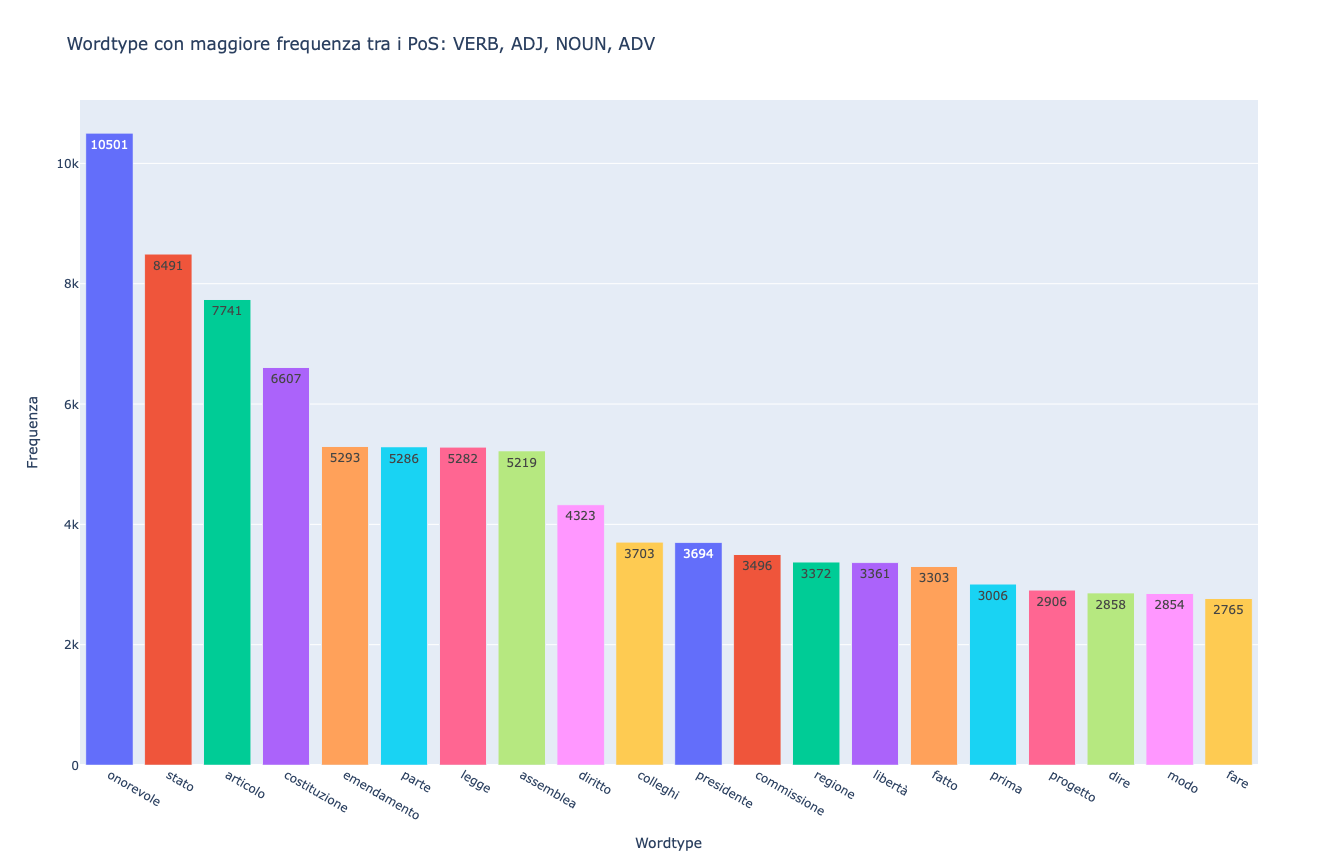
\includegraphics[width=1.1\linewidth]{newplot.png}
    \caption{20 parole più frequenti nel corpus}
    \label{fig:enter-label}
\end{figure}


Come mostra la Figura 1, si nota subito che il lessico emerso come maggiormente frequente sia in prima istanza rappresentativo del sottocodice del discorso parlamentare e dell’orazione politica. Il riferimento alle espressioni come \textit{onorevole}, \textit{presidente}, \textit{colleghi}, come primario interlocutore/i, espresso con un vocativo, compare come incipit nella quasi totalità delle relazioni. Risulta particolarmente significativo il linguaggio relativo al testo costituzionale oggetto di discussione: \textit{articolo}, \textit{costituzione}, \textit{emendamento}, \textit{parte}, \textit{legge}. 
Verbi come \textit{dire} e \textit{fare}, risultano ampiamente impiegati, in virtù del loro valore polifunzionale, nelle espressioni che raccontano il \textit{farsi} della costituzione, ovvero ciò che stava avvenendo in quei mesi nell’aula parlamentare e di cui i costituenti hanno profonda coscienza.  Particolarmente interessante, oltre all’elevato impiego del termine astratto \textit{libertà} – coerente con i valori fondanti della Costituzione –, è l’ampia frequenza del termine \textit{regione}, spia della rilevanza della riflessione attorno all’autonomia regionale nella discussione, spesso trascurato nelle riflessioni sul testo costituzionale. Questo tema, in particolare, emergerà tramite analisi più sofisticate nell’ambito del progetto.


\section{Il discorso nel tempo}

Nell'ottica di affinare l'analisi statistico frequenziale si è proceduto facendo emergere, seguendo l'andamento temporale dei lavori dell'Assemblea Costituente da marzo a dicembre, il lessico specifico e proprio di ogni mese che scandisce la discussione. Il lessico proprio e rappresentativo di ogni mese è stato ottenuto tramite metriche TF-IDF. Ottenendo così non le parole più frequenti per ogni mese, ma quelle che maggiormente appaiono nel mese che si sta analizzando e meno nel corpus complessivo. 

\begin{figure}[H]
    \centering
    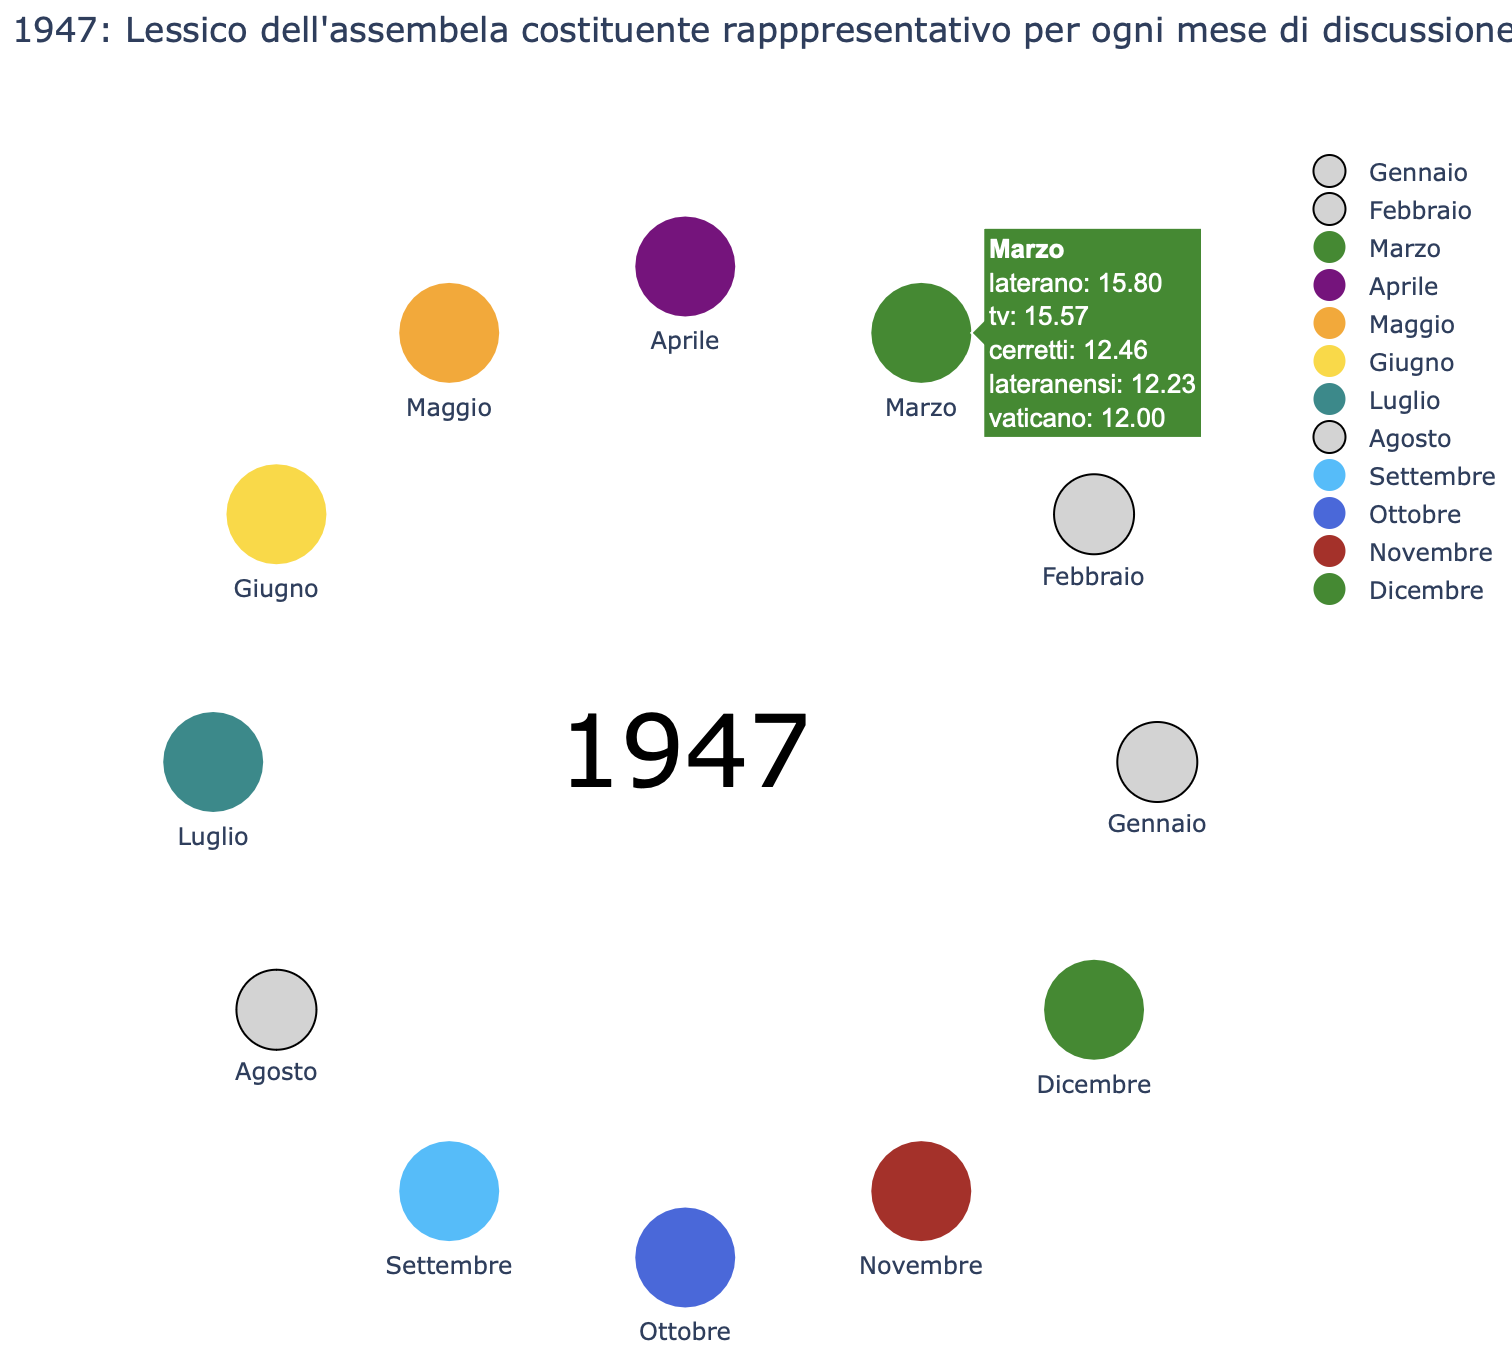
\includegraphics[width=0.5\linewidth]{TF_IDF.png}
    \caption{Parole specifiche secondo la metrica TF-IDF}
    \label{fig:enter-label}
\end{figure}

Vista l'impossibilità di essere esaustivi in questa sede, si analizzerà qui - a titolo esemplificativo uno dei mesi di discussione più significativi, per rendere conto di come il lessico specifico, ottenuto con questa metrica e con questa modalità, sia rappresentativo delle tematiche discusse. 

\begin{figure}[H]
    \centering
    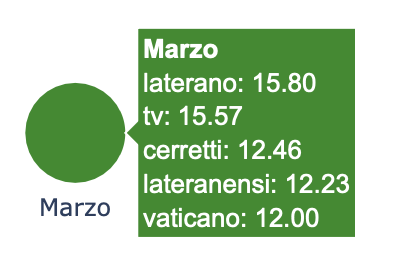
\includegraphics[width=0.5\linewidth]{marzo.png}
    \caption{Parole specifiche del mese di marzo 1947}
    \label{fig:enter-label}
\end{figure}

Come mostrato in Figura 3, le parole specifiche delle relazioni pronunciate nel mese di Marzo riguardano la regolazione dei rapporti tra Stato e Chiesa. Se infatti le relazioni dal 4 marzo , ovvero l’apertura dei lavori dell’assemblea plenaria, all’11 marzo afferiscono a un ampio dibattito attorno al progetto generale di Costituzione, sul solco della natura del carattere di “compromesso” con cui stava nascendo la carta costituzionale, la discussione si è spostata alla regolazione dei rapporti tra Stato e Chiesa. Diverse relazioni si spendono circa il riconoscimento da dare ai Patti Lateranensi, infatti, tra le parole con valore di rappresentatività TF-IDF maggiore, troviamo proprio \textit{lateranensi}. Da queste settimane di discussione emerge l'attuale art. 7 della Costituzione, approvato tra il 25 e il 26 marzo 1947: 

\textit{{Lo Stato e la Chiesa cattolica sono, ciascuno nel proprio ordine, indipendenti e sovrani. I loro rapporti sono regolati dai Patti Lateranensi. Le modificazioni dei Patti, accettate dalle due parti, non richiedono procedimento di revisione costituzionale.}}

La discussione su questi punti infiamma un acceso dibattito e richiede di giungere a un compromesso tra le varie forze politiche, poiché la preminenza connessa al cattolicesimo e i privilegi per la chiesa e le sue strutture erano difficilmente accettabili da una cultura di matrice laica. Da parole rappresentative  come \textit{Cerretti}, ovvero il rappresentante del Vaticano in dialogo con Vittorio Emanuele Orlando dopo la prima guerra mondiale per un primo tentativo di concordato, si evince la profondità di sguardo storico che è propria della discussione, oggetto di una grande diatriba, neppure oggi del tutto spenta.

\newpage
\section{I temi della discussione costituzionale: un'indagine attraverso Topic Modelling}


Tecniche di analisi di Topic Modelling hanno permesso di identificare in modo induttivo i temi predominanti all'interno del corpus documentale. L'infografica, mostrata in figura 4, consente di indagare interattivamente le parole chiave che definiscono ciascun tema.

A partire dalle parole associate a ogni topic, è possibile ipotizzare che il corpus sia composto dai seguenti temi predominanti:

\begin{itemize}
    \item 1 \(\Rightarrow\)\textbf{Attività parlamentare}
    \item 2 \(\Rightarrow\)\textbf{Autonomia regionale}
    \item 3 \(\Rightarrow\)\textbf{Libertà individuale e sistema educativo }
    \item 4 \(\Rightarrow\)\textbf{Principi costituzionali }
    \item 5 \(\Rightarrow\)\textbf{Sistema giudiziario}
    \item 6 \(\Rightarrow\)\textbf{Diritti sociali dei lavoratori}
    \item 7 \(\Rightarrow\)\textbf{Diritto di famiglia e diritti civili}
    \item 8 \(\Rightarrow\)\textbf{Politica e democrazia nel sistema repubblicano}
\end{itemize}

\begin{figure}[H]
    \centering
    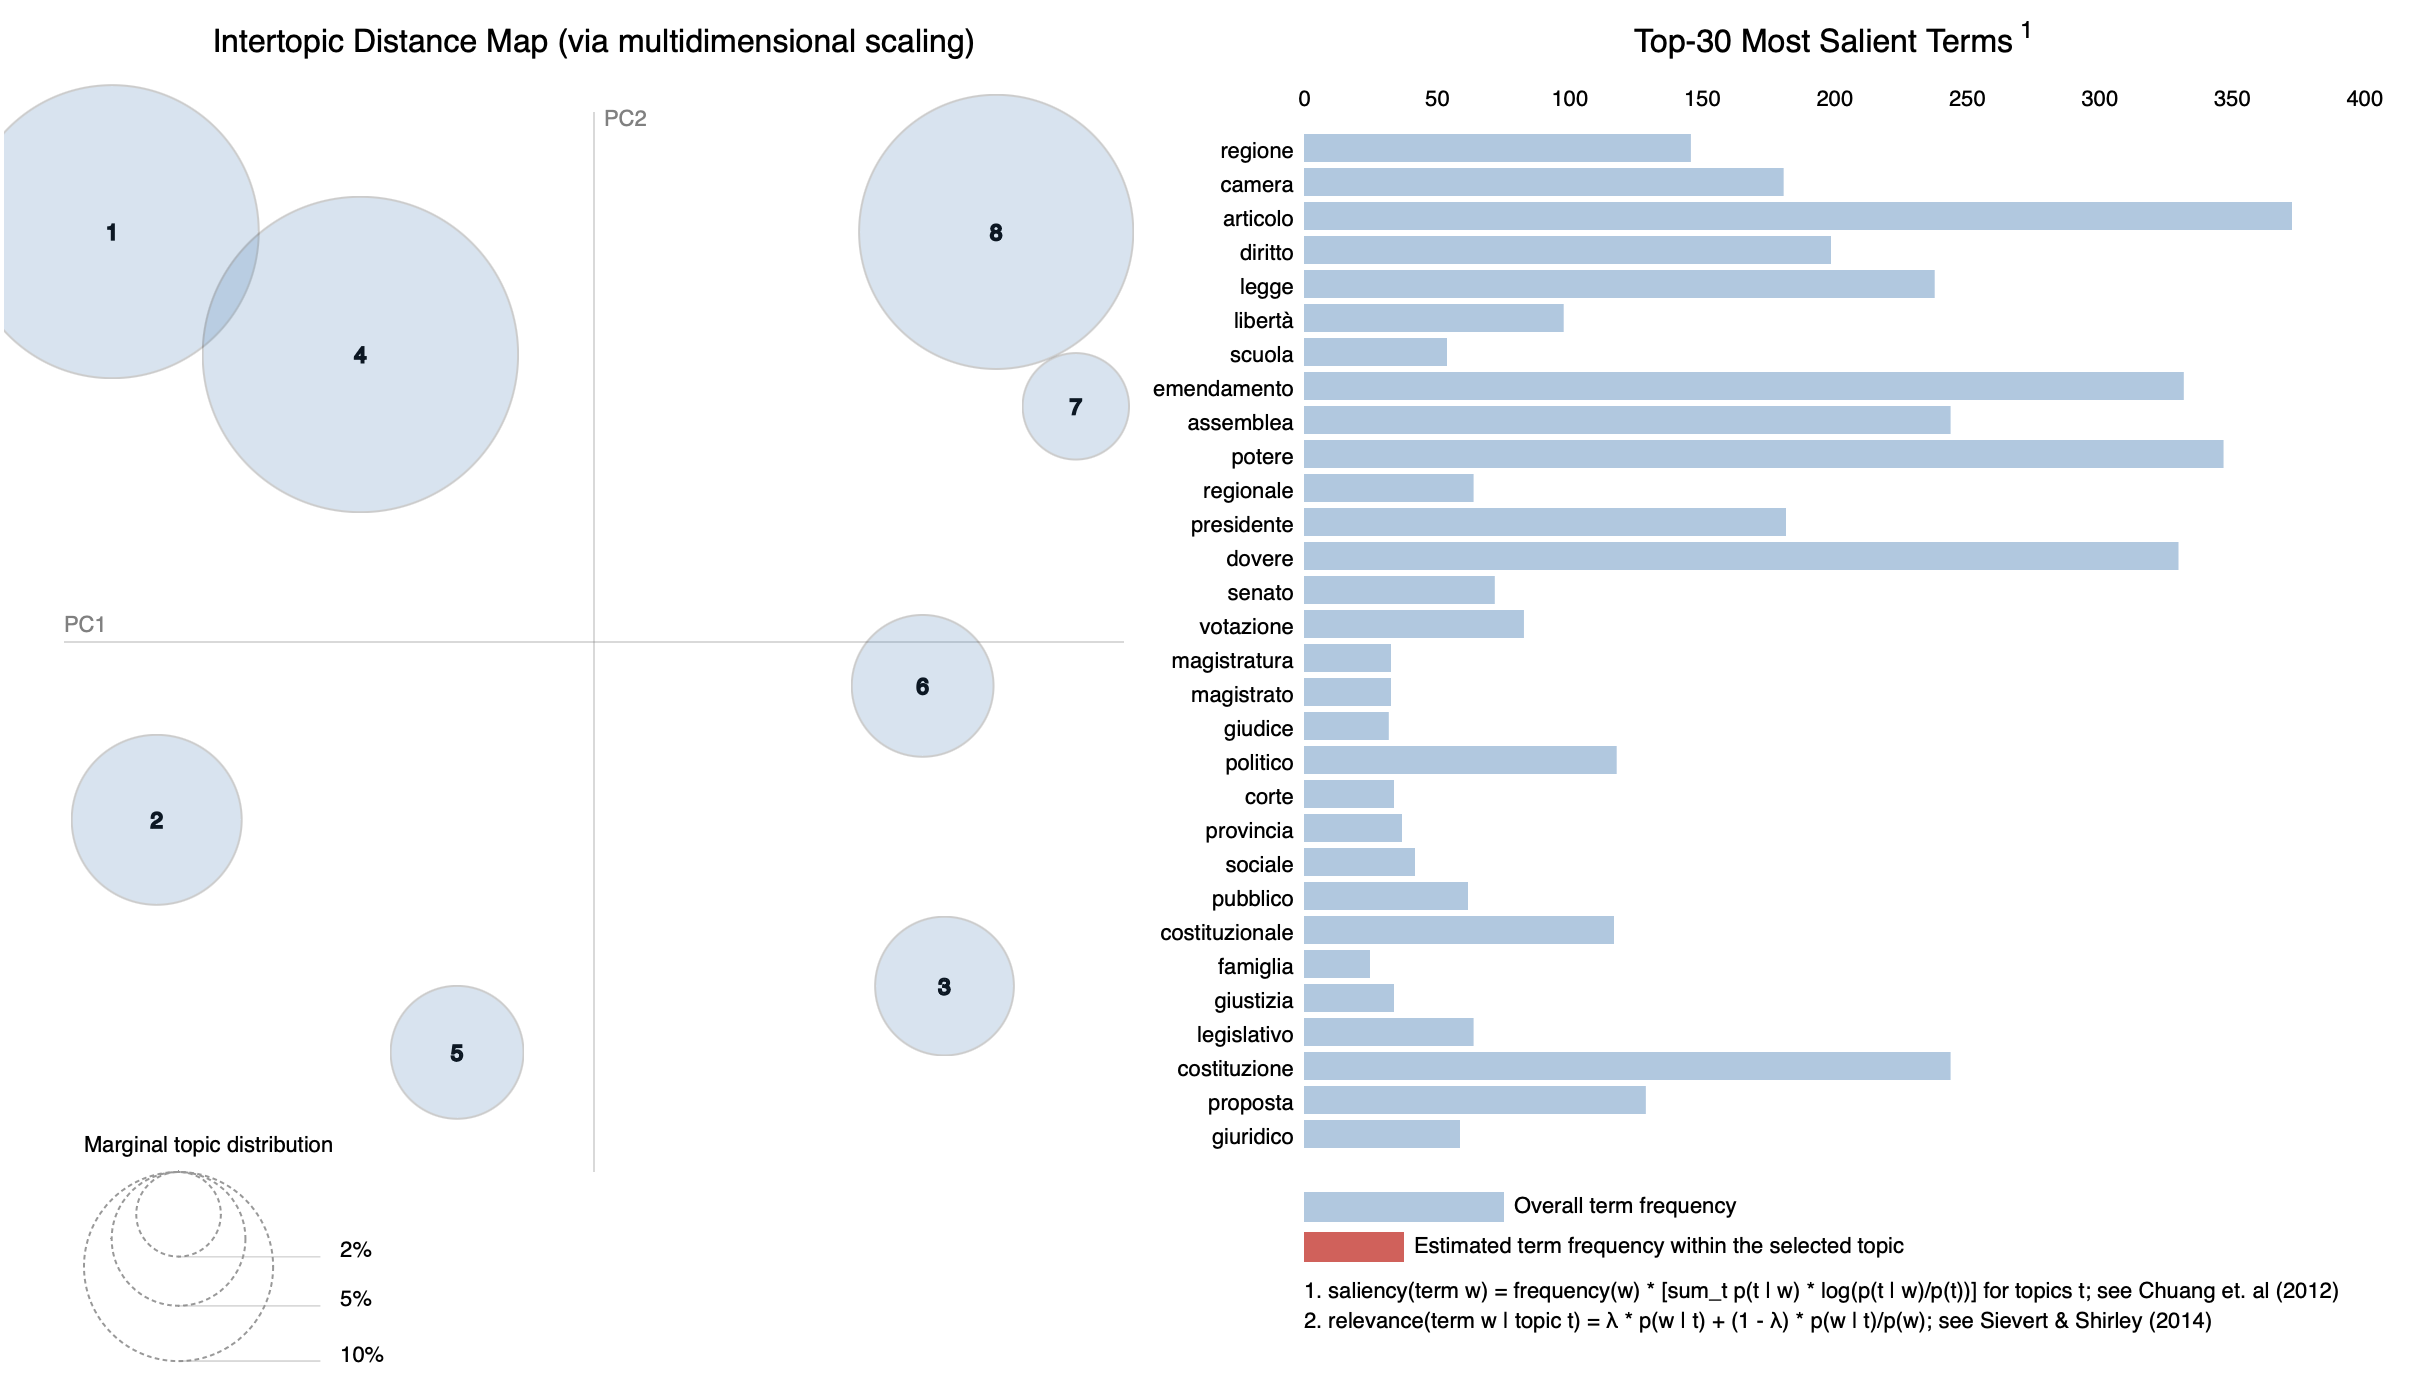
\includegraphics[width=1\linewidth]{topic_model.png}
    \caption{Topic Model}
    \label{fig:enter-label}
\end{figure}

A titolo esemplificativo, l'analisi del topic 7 consente di approfondire la pervasività di questo tema nel dibattito e di valutare l'importanza degli elementi linguistici che emergono.

\begin{figure}
    \centering
    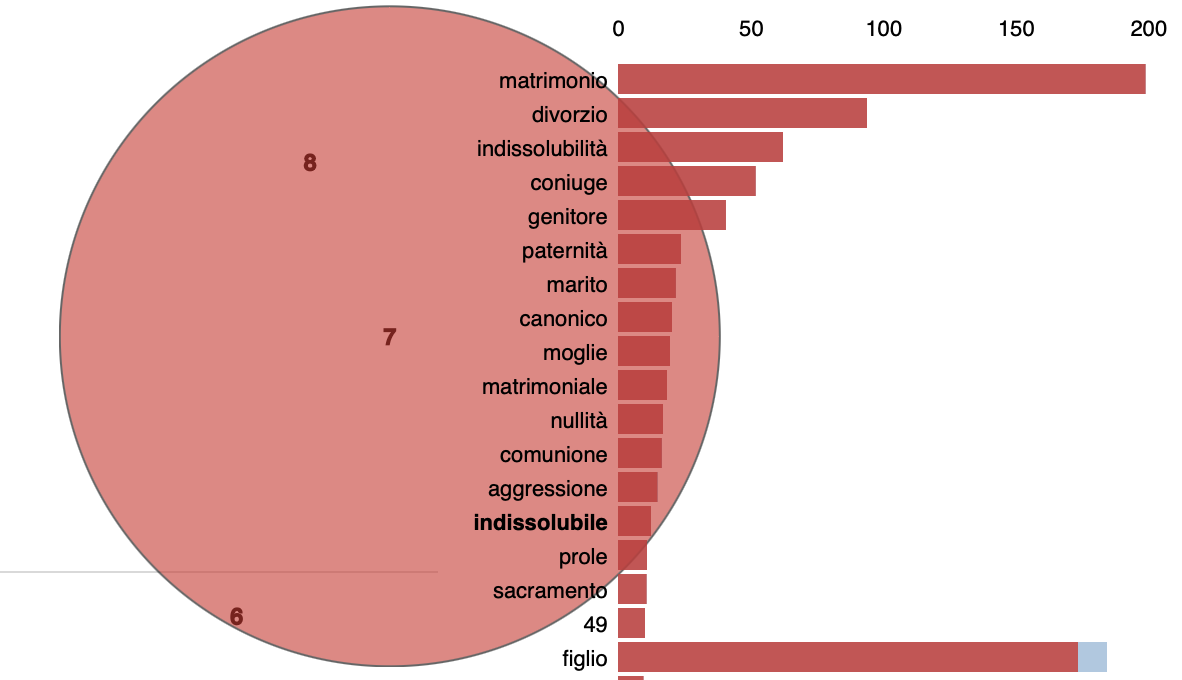
\includegraphics[width=1\linewidth]{topic_7.png}
    \caption{Topic 7}
    \label{fig:enter-label}
\end{figure}

Indagando il corpus osserviamo la ricorrenza della locuzione \textit{matrimonio indissolubile} in 55 relazioni, una chiara manifestazione della centralità di tale concetto nel dibattito costituzionale. La questione del matrimonio indissolubile appare come un nodo cruciale all'interno della discussione sulla famiglia e sui diritti civili, come esemplifica una frase della proposta di testo costituzionale discussa in Assemblea "\textit{La Repubblica riconosce i diritti della famiglia come società naturale fondata sul matrimonio indissolubile.}"


Un momento decisivo della discussione si è verificato la notte del 23 aprile, quando l'Assemblea Costituente ha affrontato la votazione di un emendamento proposto dal deputato socialdemocratico Grilli, volto a sopprimere l'aggettivo "indissolubile" dopo la parola matrimonio, nel primo comma dell'articolo. La votazione ha visto la partecipazione di 385 membri, con una maggioranza di 193 voti favorevoli e 191 contrari, segnando un risultato che ha lasciato un margine minimo: un solo voto di scarto rispetto al quorum richiesto. In questo contesto, la Costituzione repubblicana ha sancito la possibilità che il matrimonio non fosse necessariamente indissolubile. 

L'eliminazione del termine \textit{indissolubile} ha avuto implicazioni più ampie, contribuendo ad aprire la strada a un riconoscimento più ampio delle libertà individuali, rendendo il divorzio possibile costituzionalmente. Diventato legge solo nel 1970, con l'approvazione della legge Fortuna-Baslini, il divorzio è stato possibile proprio grazie all'eliminazione dell'attributo indissolubile dal sostantivo matrimonio nella discussione sulla Costituzione. 

Dati come questo dimostrano l’importanza di tecniche di topic modelling e analisi linguistica basate su Natural Language Processing (NLP), che permettono di rivelare lessemi fondamentali nel dibattito costituzionale che, altrimenti, potrebbero sfuggire a un’analisi più superficiale. L’analisi di un corpus documentale, come quello dell’Assemblea Costituente, permette infatti di identificare parole e concetti che sono stati discussi ma che non sono stati infine inseriti nel testo ufficiale. In questo caso, la parola indissolubile, pur essendo centrale nel dibattito, è assente dalla Costituzione, ma la sua rilevanza nella discussione è fondamentale per comprendere l’evoluzione storica della legislazione sul matrimonio e il divorzio.

Tale approccio, che va oltre un’analisi impressionistica e si basa su strumenti avanzati di analisi linguistica, consente di ottenere una comprensione più profonda e oggettiva dei temi trattati, anche su un piano storico e qualitativo. Questo tipo di analisi permette, quindi, di tracciare legami significativi tra scelte politiche e le dinamiche linguistiche che hanno influenzato la stesura del testo costituzionale.


\section{Bibliografia}

\begin{itemize}
    \item Atti della Assemblea Costituente. Roma, Tipografia della Camera dei deputati, 1970.
    \item Vittorio Caporrella, La famiglia nella Costituzione italiana. La genesi dell'articolo 29 e il dibattito della Costituente. Storicamente, 2010.
    \item Fiamma Lussana, Famiglia e indissolubilità del matrimonio nel dibattito all'assemblea costituente. Studi Storici, 2014.
    \item Paolo Pombeni, La questione costituzionale in Italia. Il Mulino, Bologna, 2016.
    \item Fulvio Cortese, Corrado Caruso, Stefano Rossi, Immaginare la Repubblica. Mito e attualità dell'Assemblea Costituente. Franco Angeli, Milano, 2018. 
\end{itemize}
\end{document}
